\documentclass{article} % For LaTeX2e
\usepackage{nips14submit_e,times}
\usepackage{amsmath}
\usepackage{hyperref}
\usepackage{url}
\usepackage{graphicx}

%\documentstyle[nips14submit_09,times,art10]{article} % For LaTeX 2.09

\title{Reading Minds : Identifying read words using images of brain activity}
\subtitle{CSE 546: Final Project Report}
\author{
Tomasz Sarkedja \\
Physics Department\\
University of Washington\\
\texttt{tomaszs@uw.edu} \\
\And
Stella Stylianidou \\
Physics Department\\
University of Washington\\
\texttt{stellast@uw.edu} \\
}


\newcommand{\fix}{\marginpar{FIX}}
\newcommand{\new}{\marginpar{NEW}}

\nipsfinalcopy % Uncomment for camera-ready version

\begin{document}


\maketitle

\begin{abstract}
Machine learning techniques are often used to decipher brain images experiments and find whether there are relationships between fMRI data and variables of interest. In this study we show that we can predict the words a participant is reading using the brain activation patterns measured via FMRI, thereby showing that fMRI data contain information about the words read. We are able to predict the relationship between the FMRI's with a set of 218 semantic features. Following that we use the semantic feature scores to guess the words the participant was looking with a success rate of 80\%, which is at the success rate found in literature. 

\end{abstract}

\section{Introduction}

Humans have always sought to understand the brain better. Functional magnetic resonance imaging (FMRI), which is an imaging procedure that measures brain activity by detecting changes associated with blood flow, has been a vital component in medical diagnosis, but also in improving our understanding of the human brain and its biology. The information in an FMRI scan is complicated, dense, and interpreting it requires analysis of complex, multivariate data[http://www.sciencedirect.com/science/article/pii/S1053811908012263]. With the advent of machine learning it is now possible to find relationships between FMRI scans and human actions or thoughts that were not possible before, and thus proove that the fMRI data contain information about those.

In this work we seek to find a relationship between FMRI scans and words. We use 'semantic features', which are properties which we use to characterize words. We use the mappings established between words and semantic features to predict the word given an FMRI. Our data consists of 60 words and their relationship to 216 semantic features. We use 360 FMRI images consisting of 20,000 voxels. Our current model relates each semantic feature separately to the brightness of the voxels. The obtained parameters can then be used to predict the value of each of the semantic features for a given FMRI image, and the predicted semantic features values can be used to identify the word. This method can be used to predict words for which we know semantic features but our model has not be trained on.



\section{Methods}
Because FMRI scans are expensive the amount of data one can obtain is limited. This makes training our model difficult because the amount of training data (360) is significantly smaller than the dimensionality of the problem (20,000 voxels). Currently we are using linear regression with L1 regularization (Lasso). We expect a strong reduction in the bias of our trained parameters over non-regularized linear regression. The Lasso is used to predict values of 218 semantic features from our FMRI's. The semantic feature values for the training data are obtained via questionarre with responses given ratings between 1-5 by the test subject. These data are then centered and normalized.



\subsection{Lasso}

To obtain the parameters that relate the value of a semantic feature to the voxels in the brain images we use linear regression with Lasso. Lasso, as described in Tibshirani (1996) [1], constrains the L1 norm, thereby shrinking some weights to exactly zero. This technique therefore obtains sparse solutions, which can be useful in the case that the amount of data is much smaller than the dimensionality of the problem (as in this case), or if we expect that few voxels are related to each word. 

To estimate the weights with Lasso we minimize the following function :

\begin{align*}
w_{Lasso} = argmin \{|| Y - Xw ||^2 + \lambda|w|\}
\end{align*}



\section{Results}


\subsection{Obtaining the best lambda}
In order to choose a $\lambda$ suitable for our dataset we used pathwise optimization [2]. In pathwise optimazion we start with a high value for  $\lambda$ and solve the optimization for a decreasing series of lambdas using the previous results for our weights. We finally choose the $\lambda$ with the smallest root mean square error on a validation set, which is a subset partitioned from our training data. Since the semantic features consist of similar realtionships, we attempted to choose the best $\lambda$ for our dataset using one of the semantic features. 250 FMRI images were used to train our dataset and 50 were used as validation data. We started from maximum lambda calculated as $2 * max (|X^T.(y - <y>)|)$ and decreased the $\lambda$ by multiplying by 0.8 in each iteration. Choosing the lambda using this method on different semantic features obtained similar values for all features, but larger values than expected (~134). In figure 1, we shown the root mean square error on the training data and validation data versus different $\lambda$. This large value of $\lambda$ creates a very sparse solution and sets most of the features to 0. The reason behind the large value of lambda may be due to the nature of the data, or the large dimensionality compared to the amount of training data we have.



\begin{figure}[h]
\begin{center}
%\framebox[4.0in]{$\;$}
%\fbox{\rule[-.5cm]{0cm}{4cm} \rule[-.5cm]{4cm}{0cm}}
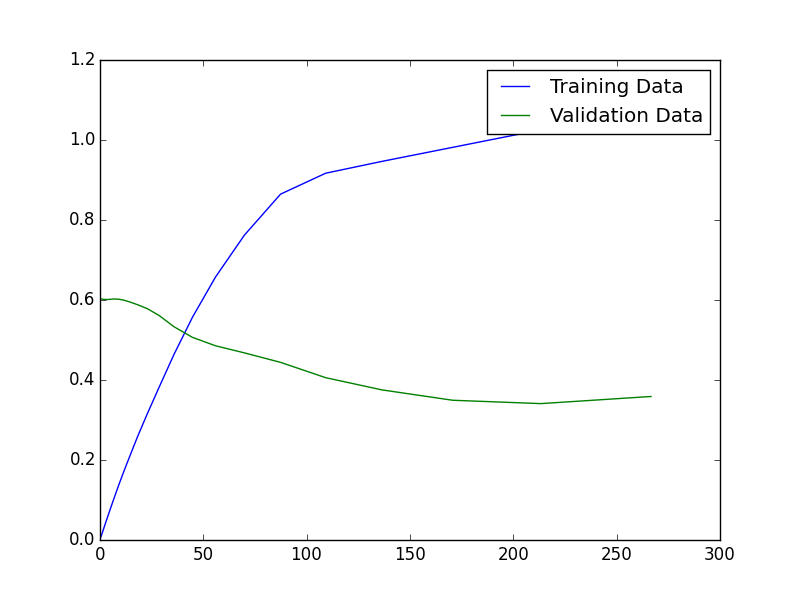
\includegraphics[scale=0.5]{trainvalidlambda}
\end{center}
\caption{Training lambdas on the first semantic feature on 250 data, and using 50 FMRI
images as a validation test. Horizontal axis: value of lambda. Vertical axis: RMSE. The data suggest strong overfitting on our training set.}
\end{figure}

Following this initial test we tried cross validating our choice of $\lambda$. For each step we chose 60 FMRIs to be our validation set and then used the remaining 240 FMRI's as our training set. We still used holdout set of 60 for testing. The results were largely indistinguishable from performing single step validation, except that one of the $\lambda$ returned was much smaller than the rest. This discrepancy suggests that our current method of choosing a lambda is ill informed, probably due to the homogeneity of our semantic feature data. Currently we believe that it may be necessary to choose a $\lambda$ based on several semantic features, because doing so would resolve the problem of the homogeneity of the semantic features.



\subsection{Results on the test data}

The task for our model is simplified somewhat because the model need only choose between two words given an FMRI. Using a $\lambda$ of 134 as a starting point, obtained from training on the first semantic feature, we trained each of the other semantic feature for $\lambda$ 134 +/- 5 and chpose the $\lambda$ value that had the lowest RMSE on the validation set. With the obtained weights we predicted the values for the 216 semantic features for each of the test cases. The predicted semantic feature values were then compared to the semantic features of the two given words. The word for which the semantic features have the smallest distance from the predicted semantic features was chosen. 

For this value of $\lambda$ our results were close to random with only 52\% of the words guessed correctly (31 out of 60), indicating that the weights predicted are not satisfactory for the prediction of the semantic features.

We also run our algorithm with the lambdas suggested in the CSE599 homework where the values are (0.05,0.1,0.15,0.2,0.25,0.3,0.35,0.4), but again obtained results that are essentially random with 49\% of the words guessed correctly. The root mean square error on our training data set was \~0.25, where as on our test data set it was of the order of 22000. We're currently investigating issues with our lasso implementation, but the poor results obtained thus and the seeming overfitting of our training data are making us consider other models.


\section{Future Directions}

The predictive power of our algorithm is not at where we would like it to be. Some ideas for future directions to improve the predictive power are the following :

\subsection{Principal Component Analysis}
The difficulty with this data set is that our dimensionality is many times higher than the amount of data we have. A possible way to decrease our dimensionality is to use Principal Component Analysis(PCA).  Principal Component Analysis transforms the set of observations that may be correlated into a a new basis where the set of values are linearly uncorrelated. In this new basis underlying relationships between the different voxels in our FMRI scan may be exposed. 


\subsection{Stochastic coordinate descent for lasso}
Instead of finding the minimum for all coordinates we can find the minimum for a single feature at each iteration and update that weight [3]. We can stop updating the weights when the weight converges. Implementing this method would sharply decrease our training time, allowing us to prototype new model implementations more quickly.


\subsubsection*{References}

\small{
%original lasso paper
[1] Tibshirani, R. (1996). Regression shrinkage and selection via the lasso. J. Royal. Statist. Soc B., Vol. 58, No. 1, pages 267-288

% pathwise optimization
[2] Friedman, J., Hastie, T., \& Tibshirani, R. (2010). Regularization paths for generalized linear models via coordinate descent. Journal of statistical software, 33(1), 1.

% stoch coordinate descent
[3] Shalev-Shwartz, S., \& Tewari, A. (2011). Stochastic methods for l 1-regularized loss minimization. The Journal of Machine Learning Research, 12, 1865-1892.
}

\end{document}
